\section{Parallel Solver for the Multidomain Electrophysiology Model}\label{sec:parallel_solver_multidomain}

After the details on the parallel partitioning and solvers for the fiber based electrophysiology model have been discussed in \cref{sec:parallel_partitioning_and_sampling_of_the,sec:parallel_partitioning_for_fiber_based}, we now consider the multidomain based model of electrophysiology, which includes electric conduction in the body fat layer. The class for the implicit solver within the operator splitting is the \code{MultidomainWithFatSolver} class, which has been introduced in \cref{sec:exemplary_usage_2}.

\subsection{Construction and Partitioning of the Mesh}

The mesh used in this solver is a composite mesh of type \code{Mesh::CompositeOfDimension<D>}, as introduced in \cref{sec:composite_meshes}. \Cref{fig:structured_grid_n_nodes} shows the layout how the mesh of the body fat domain $\Omega_B$ is connected with the mesh of the muscle domain $\Omega_M$. The muscle and body meshes have $N_x^\text{el} \times N_y^\text{el} \times N_z^\text{el}$ and $(N_x^\text{el}+ N_y^\text{el}) \times N_\text{fat}^\text{el} \times N_z^\text{el}$ elements, respectively. Only the muscle mesh has been generated from medical imaging data by the pipline given in \cref{sec:generation_of_meshes_for_multiscale}. The fat mesh is created on top of the muscle mesh geometry and has to use the same number of elements as the muscle mesh for compatibility in the composite mesh. Only the physical thickness of the adipose tissue layer and the corresponding number $N_\text{fat}^\text{el}$ of elements in radial direction have to be specified.  (The mesh generation step is implemented in the script \code{create_fat_layer.py}.) 

% fat layer mesh and partitioning
\begin{figure}
  \centering%
  \def\svgwidth{0.6\textwidth}
  \input{images/implementation/structured_grid_n_nodes.pdf_tex}%
  \caption{Layout of the composite 3D mesh for the multidomain model with fat layer. The orange elements belong to the mesh of the muscle domain $\Omega_M$, the yellow elements are added on top to represent the body domain $\Omega_B$.}%
  \label{fig:structured_grid_n_nodes}%
\end{figure}%

\Cref{fig:multidomain_matrix_mesh} shows such as composite mesh.
The muscle mesh is based on a dataset of $13\times 13$ fibers with \num{1481} nodes per fiber. This fine mesh is sampled as described in \cref{sec:algorithm_for_partitioning_and_sampling} with stride values of $3,3$ and $20$ in $x,y$ and $z$ directions and \code{distribute_nodes_equally=True}. In result, we get $N_x^\text{el} \times N_y^\text{el} \times N_z^\text{el} = 5 \times 4 \times 75$ elements.
The fat mesh consists of a $\SI{1}{\centi\meter}$ adipose tissue layer with $N_\text{fat}^\text{el}=4$ elements. The muscle and fat meshes have \num{2280} and \num{3800} dofs, yielding a 

% comment about parallelization
The partitioning of the composite mesh into $n_x \times n_y \times n_z$ subdomains cannot be chosen arbitrarily. The reason is that both the muscle and the body fat mesh have to be partitioned to the same number of processes. 
If, e.g., a partitioning of $n_x=n_y=2$ is chosen, the cube in \cref{fig:structured_grid_n_nodes} gets divided by one horizontal planar cut and one vertical planar cut. This divides the orange muscle mesh into four subdomains as expected. The yellow body fat mesh, however, is only partitioned to three of the four processes as there are no yellow elements below the horizontal cut and left of the vertical cut.

Thus, a valid partitioning can only be created if either $n_x$ or $n_y$ is set to one. Because there is no restriction on $n_z$, the total mesh can still be partitioned in two dimensions to a product of subdomains, either as $1 \times n_y \times n_z$ or as $n_x \times 1 \times n_z$.
The example mesh in \cref{fig:multidomain_matrix_mesh} is partitioned to $2 \times 1 \times 2$ subdomains as shown by the different colors.

% scenario_name: matrix,  n_subdomains: 2 1 2,  n_ranks: 4,  end_time: 0.002
% dt_0D:           1e-03    multidomain solver:         1000 it. of gmres (10000 it. of gmres), lumped mass matrix: False, initial guess: previous solution
% dt_multidomain:  1e-03    multidomain preconditioner: euclid (euclid), symmetric precond.: True
% dt_splitting:    1e-03    theta: 1.0, solver tolerances, abs: 1e-15, rel: 1e-15
% fiber_file:              ../../../input/left_biceps_brachii_13x13fibers.bin
% fat_mesh_file:           ../../../input/left_biceps_brachii_13x13fibers.bin_fat.bin
% cellml_file:             ../../../input/hodgkin_huxley_1952.c
% firing_times_file:       ../../../input/MU_firing_times_always.txt
% ********************************************************************************
% 4 ranks, partitioning: x2 x y1 x z2
%   sampling 3D mesh with stride 3 x 3 x 20 
%   distribute_nodes_equally: True
%     linear 3D mesh    nodes global: 6 x 5 x 76 = 2280, local: 3 x 5 x 38 = 570
%     linear 3D mesh elements global: 5 x 4 x 75 = 1500, local: 3 x 4 x 38 = 456
%     fat mesh, n points total:    3800 (10 x 5 x 76), (per process: 3 x 5 x 38 = 570)
% 
\begin{figure}
  \centering%
  \includegraphics[width=\textwidth]{images/implementation/multidomain_matrix_mesh.png}%
  \caption{Composite mesh of the multidomain example, partitioned to four processes.}%
  \label{fig:multidomain_matrix_mesh}%
\end{figure}%

\subsection{Structure of the System Matrix}

The \code{MultidomainWithFatSolver} class uses nested \code{FiniteElementMethod} classes to describe the anisotropic electric conduction in the muscle domain and the isotropic electric conduction in the fat domain.
The system matrix for the system of equations is given in \cref{eq:discretized_multidomain_body2} in \cref{sec:discretization_body_domain}. 
The solver calculates the matrix block entries using the stiffness and mass matrices computed by the nested \code{FiniteElementMethod} classes.

\Cref{fig:original_matrix} shows the location of non-zeros in the resulting sparse matrix for three MUs. The matrix blocks are indicated by boxes and can be identified by comparison with \cref{eq:discretized_multidomain_body2}. In this visualization, it may seem that most of the blocks only have three non-zero entries per row, however, the actual number is higher with a maximum of 27 entries, as the Finite Element ansatz function of a node in the 3D mesh has overlapping support with the ansatz functions of other nodes in a $3\times 3 \times 3$ grid.
The actual non-zero structure per block is close to the example shown in \cref{fig:sparsity_pattern}.

The colors in \cref{fig:original_matrix} correspond to the four processes, as defined in the partitioned mesh in \cref{fig:multidomain_matrix_mesh}. 
The entries in every block are all partitioned in the same way to the four processes, as given by the partitioning of the nested \code{FiniteElementMethod} classes. The data structure for this layout is the \code{MATNEST} type of PETSc. 

However, to be able to apply the multitude of PETSc solvers to this linear system, the matrix has to be transferred to the canonical parallel matrix layout of PETSc that groups all dofs of the subdomains together. As this conversion is not available in PETSc, it is done in OpenDiHu by reordering the dofs and, in consequence, the matrix entries. The same permutation is applied to the rows and the columns of the matrix. The result of this operation is shown in \cref{fig:reordered_matrix}. It can be seen that the portions for each process are now consecutive matrix rows. The non-zero structure within each process resembles the global matrix structure of the original matrix.

% multidomain uses two fem objects, parallel partitioning
% reorder matrix entries
% for 16 processes scenario

\begin{figure}%
  \centering%
  \begin{subfigure}[t]{0.49\textwidth}%
    \centering%
    \includegraphics[width=\textwidth]{images/implementation/original_matrix.png}
    \caption{Original matrix layout}%
    \label{fig:original_matrix}%
  \end{subfigure}
  \,
  \begin{subfigure}[t]{0.49\textwidth}%
    \centering%
    \includegraphics[width=\textwidth]{images/implementation/reordered_matrix.png}
    \caption{Reordered matrix layout}%
    \label{fig:reordered_matrix}%
  \end{subfigure}
  \caption{Nonzero structure of the system matrix of the multidomain problem.}%
  \label{fig:original_reordered_matrix}%
\end{figure}%

\subsection{Properties of a Diagonal Block-Matrix for the Preconditioner}
With the reordered matrix, the linear system can now be solved using almost any preconditioner and linear solver of the PETSc framework. 
For the construction of the preconditioner $\mathcal{P}$ with left preconditioning matrix $P=\mathcal{P}(A)$, we can either use the system matrix $A$ or provide a different matrix $A'$. The preconditioned linear system $P^{-1}A$ should have a smaller condition number than $A$ and, thus, solving the preconditioned system iteratively should be significantly faster than the original $A$ system.

To compute the condition number of the system matrix $A$, we determine its spectrum. \Cref{fig:eigenvalues} shows the real parts of all eigenvalues of $A$. The imaginary parts vanish for almost all eigenvalues. The matrix is singular with one zero-eigenvalue. This property corresponds to the fact that the membrane potential in the problem is abitrary with respect to a constant offset. The singular problem can be solved using appropriate iterative solvers.

% eigenvalues, spectrum, condition number is bad -> preconditioning
The real parts of the eigenvalues are all negative, which is in line with the fact that the model consists of a combination of several diffusion problems. The progression in \cref{fig:eigenvalues} shows a large difference between the largest and the smallest eigenvalues. The condition number of $A$ can be computed by $\textrm{cond}(A) = |\lambda_\text{max}| / |\lambda_\text{min}| = 161.2576 / 0.0116 \approx \num{1.4e5}$. Thus, the problem is ill-conditioned and can benefit from for preconditioning. The condition number is also dependend on the spatial mesh resolution and increases for larger problem sizes.

% PETSc tutorial on preconditioning: https://www.mcs.anl.gov/petsc/meetings/2016/slides/tutorial1.pdf
\begin{figure}
  \centering%
  \includegraphics[width=0.6\textwidth]{images/implementation/eigenvalues.png}%
  \caption{Real parts of the eigenvalues sorted by magnitude and corresponding to the example in \cref{fig:multidomain_matrix_mesh}. The non-zero eigenvalue with largest and smallest absolute values are $\lambda_\text{max} = \num{-161.2576}$ and $\lambda_\text{min} = \num{-0.0116}$.}%
  \label{fig:eigenvalues}%
\end{figure}%


% the ten smallest eigenvalues of the matrix:
%     0.0000
%    -0.0116
%    -0.0183
%    -0.0193
%    -0.0204
%    -0.0211
%    -0.0222
%    -0.0229
%    -0.0235
%    -0.0239
% 
% the highest eigenvalues:
%  -161.2576
%  -157.7988
%  -153.7242
%  -151.2197
%  -149.2269
%  -144.5006
%  -143.2441
%  -142.4697
%  -139.5421
%  -139.2625

We experiment with a preconditioning matrix that only uses the diagonal blocks of the system matrix. \Cref{fig:original_diagonal_matrix} shows the non-zero structure of the resulting matrix.
As all diagonal blocks are symmetric matrices, the resulting matrix $A'$ is also symmetric in contrast to $A$. The permutation of rows and columns to obtain the parallel data layout leads to the matrix structure shown in \cref{fig:reordered_diagonal_matrix}. The permutated matrix still contains only diagonal block, because entries in the original diagonal blocks are never permutated out of this block only in their row or column but are always moved by the same permutation in both rows and columns.
\Cref{fig:reordered_diagonal_matrix} shows that the entries on every rank are now decoupled, which potentially allows for a faster computation in the application of the preconditioner.

\begin{figure}%
  \centering%
  \begin{subfigure}[t]{0.49\textwidth}%
    \centering%
    \includegraphics[width=\textwidth]{images/implementation/original_diagonal_matrix.png}
    \caption{Original matrix layout}%
    \label{fig:original_diagonal_matrix}%
  \end{subfigure}
  \,
  \begin{subfigure}[t]{0.49\textwidth}%
    \centering%
    \includegraphics[width=\textwidth]{images/implementation/reordered_diagonal_matrix.png}
    \caption{Reordered matrix layout}%
    \label{fig:reordered_diagonal_matrix}%
  \end{subfigure}
  \caption{Nonzero structure of the symmetric preconditioner matrix of the multidomain problem.}%
  \label{fig:original_reordered_diagonal_matrix}%
\end{figure}%

\subsection{Mesh and Matrices for Higher Degrees of Parallelism}
To show the effect of a higher degree of parallelism on the matrix structure, we also partition the same mesh as in \cref{fig:multidomain_matrix_mesh} to 16 processes. The resulting partitioning of the mesh is given in \cref{fig:16_multidomain_matrix_mesh}.
\Cref{fig:16_original_reordered_diagonal_matrix} shows the non-zero structure of the system matrix and the diagonal matrices for the preconditioner. \Cref{fig:16_original_matrix} contains the original matrix structure that is permutated to the structure in \cref{fig:16_reordered_matrix}. Reordering only the diagonal blocks of the original matrix in \cref{fig:16_original_diagonal_matrix} leads to the structure in \cref{fig:16_reordered_diagonal_matrix}. 
A comparison with \cref{fig:original_reordered_diagonal_matrix} shows that the width of the non-zero band decreases for higher parallelizations.


\begin{figure}
  \centering%
  \includegraphics[width=\textwidth]{images/implementation/16_multidomain_matrix_mesh.png}%
  \caption{Partitioning to 16 processes of the mesh in the multidomain example.}%
  \label{fig:16_multidomain_matrix_mesh}%
\end{figure}%

\begin{figure}%
  \centering%
  \begin{subfigure}[t]{0.49\textwidth}%
    \centering%
    \includegraphics[width=\textwidth]{images/implementation/16_original_matrix.png}
    \caption{Original matrix layout}%
    \label{fig:16_original_matrix}%
  \end{subfigure}
  \,
  \begin{subfigure}[t]{0.49\textwidth}%
    \centering%
    \includegraphics[width=\textwidth]{images/implementation/16_reordered_matrix.png}
    \caption{Reordered matrix layout}%
    \label{fig:16_reordered_matrix}%
  \end{subfigure}
  \\
  \begin{subfigure}[t]{0.49\textwidth}%
    \centering%
    \includegraphics[width=\textwidth]{images/implementation/16_original_diagonal_matrix.png}
    \caption{Original matrix layout}%
    \label{fig:16_original_diagonal_matrix}%
  \end{subfigure}
  \,
  \begin{subfigure}[t]{0.49\textwidth}%
    \centering%
    \includegraphics[width=\textwidth]{images/implementation/16_reordered_diagonal_matrix.png}
    \caption{Reordered matrix layout}%
    \label{fig:16_reordered_diagonal_matrix}%
  \end{subfigure}
  \caption{Nonzero structure of the symmetric preconditioner matrix of the multidomain problem partitioned to 16 processes.}%
  \label{fig:16_original_reordered_diagonal_matrix}%
\end{figure}%

\begin{reproduce_no_break}
  The following commands run one timestep of the multidomain simulation with fat layer:
  \begin{lstlisting}[columns=fullflexible,breaklines=true,postbreak=\mbox{\textcolor{gray}{$\hookrightarrow$}\space}]
    cd $\$$OPENDIHU_HOME/examples/electrophysiology/multidomain/multidomain_with_fat/build_release
    mpirun -n 4 ./multidomain_with_fat ../settings_multidomain_with_fat.py matrix.py
    mpirun -n 16 ./multidomain_with_fat ../settings_multidomain_with_fat.py matrix.py
  \end{lstlisting}
  To inspect the system matrix, define a directory where the matrix should be stored. This can be done by setting the parameter \code{config[`Solvers`][`multidomainLinear}\code{Solver`][`dumpFilename`]}, e.g., to \code{`out/matrix/m`}. Then, the directory \code{out/matrix} will contain MATLAB files with the system matrix. To create the plots, open MATLAB, load the system matrix from the  respective file and open the script \code{display_matrix}\code{_entries.m}. Adjust the name of the matrix variable in the first code block, the run the desired steps of the Live Script to produce various plots.\\
  The saved file contains the system matrix already in the reordered layout shown in \cref{fig:reordered_matrix,fig:16_reordered_matrix}. The MATLAB script reverses the permutation that was applied in OpenDiHu to generate the plots of \cref{fig:original_matrix,fig:16_original_matrix}.
\end{reproduce_no_break}

% scenario_name: matrix,  n_subdomains: 4 1 4,  n_ranks: 16,  end_time: 0.002
% dt_0D:           1e-03    multidomain solver:         1000 it. of gmres (10000 it. of gmres), lumped mass matrix: False, initial guess: previous solution
% dt_multidomain:  1e-03    multidomain preconditioner: euclid (euclid), symmetric precond.: True
% dt_splitting:    1e-03    theta: 1.0, solver tolerances, abs: 1e-15, rel: 1e-15
% fiber_file:              ../../../input/left_biceps_brachii_13x13fibers.bin
% fat_mesh_file:           ../../../input/left_biceps_brachii_13x13fibers.bin_fat.bin
% cellml_file:             ../../../input/hodgkin_huxley_1952.c
% firing_times_file:       ../../../input/MU_firing_times_always.txt
% ********************************************************************************
% 16 ranks, partitioning: x4 x y1 x z4
%   sampling 3D mesh with stride 3 x 3 x 20 
%   distribute_nodes_equally: True
%     linear 3D mesh    nodes global: 6 x 5 x 77 = 2310, local: 2 x 5 x 19 = 190
%     linear 3D mesh elements global: 5 x 4 x 76 = 1520, local: 2 x 4 x 19 = 152
%     fat mesh, n points total:    3850 (10 x 5 x 77), (per process: 2 x 5 x 19 = 190)
% 

% details multidomain solver, reordering of matrix entries

% solver structure of contraction
%\begin{figure}
%  \centering%
%  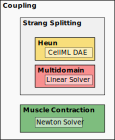
\includegraphics[width=0.5\textwidth]{images/implementation/solver_structure_contraction.pdf}%
%  \caption{solver structure}%
%  \label{fig:prestrech1b}%
%\end{figure}%


\section{CellML Adapter} % -> split into user and developer part
% code generator
% simd
% gpu

\section{Solid Mechanics Solver}
% load steps, initalization in the dynamic case


\section{Mapping Between Meshes}

% mapping between meshes
% mapping between meshes, source dofs


\section{Output Writers}
% output writers
% verschiedene output writer für das gleiche Faser-Modell


